% or aspectratio=43
\documentclass[aspectratio=169,handout]{beamer}

% remove this line for an english presentation
%\usepackage{ngerman}

% Optional arguments (separate by comma):
% darkmode			- Black background and white font
% imagetitlepage	- Adds the images defined in \titlegraphic to the title page
\usepackage[imagetitlepage]{lgdv/lgdv_beamer}

\usepackage{mdframed}
\usepackage{siunitx}
\usepackage{xcolor}
\graphicspath{{images/}}


\newcommand\ytl[2]{
	\parbox[b]{8em}{\hfill{\color{cyan}\bfseries\sffamily #1}~$\cdots\cdots$~}\makebox[0pt][c]{$\bullet$}\vrule\quad \parbox[c]{10.5cm}{\vspace{7pt}\color{red!80!black!80}\raggedright\sffamily #2\\[7pt]}\\[-3pt]}


\subtitle{AGPhys WS 20/21                                                                                                 }
\title{Profiling and Optimizing CUDA Kernels}
\author[Darius Rückert]{Darius Rückert}
\date{\today}

\titlegraphic
{
	\begin{figure}[!h]
					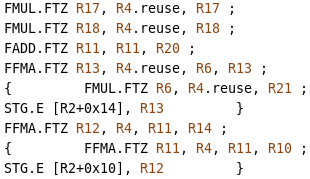
\includegraphics[height=.3\textheight]{sass2}
						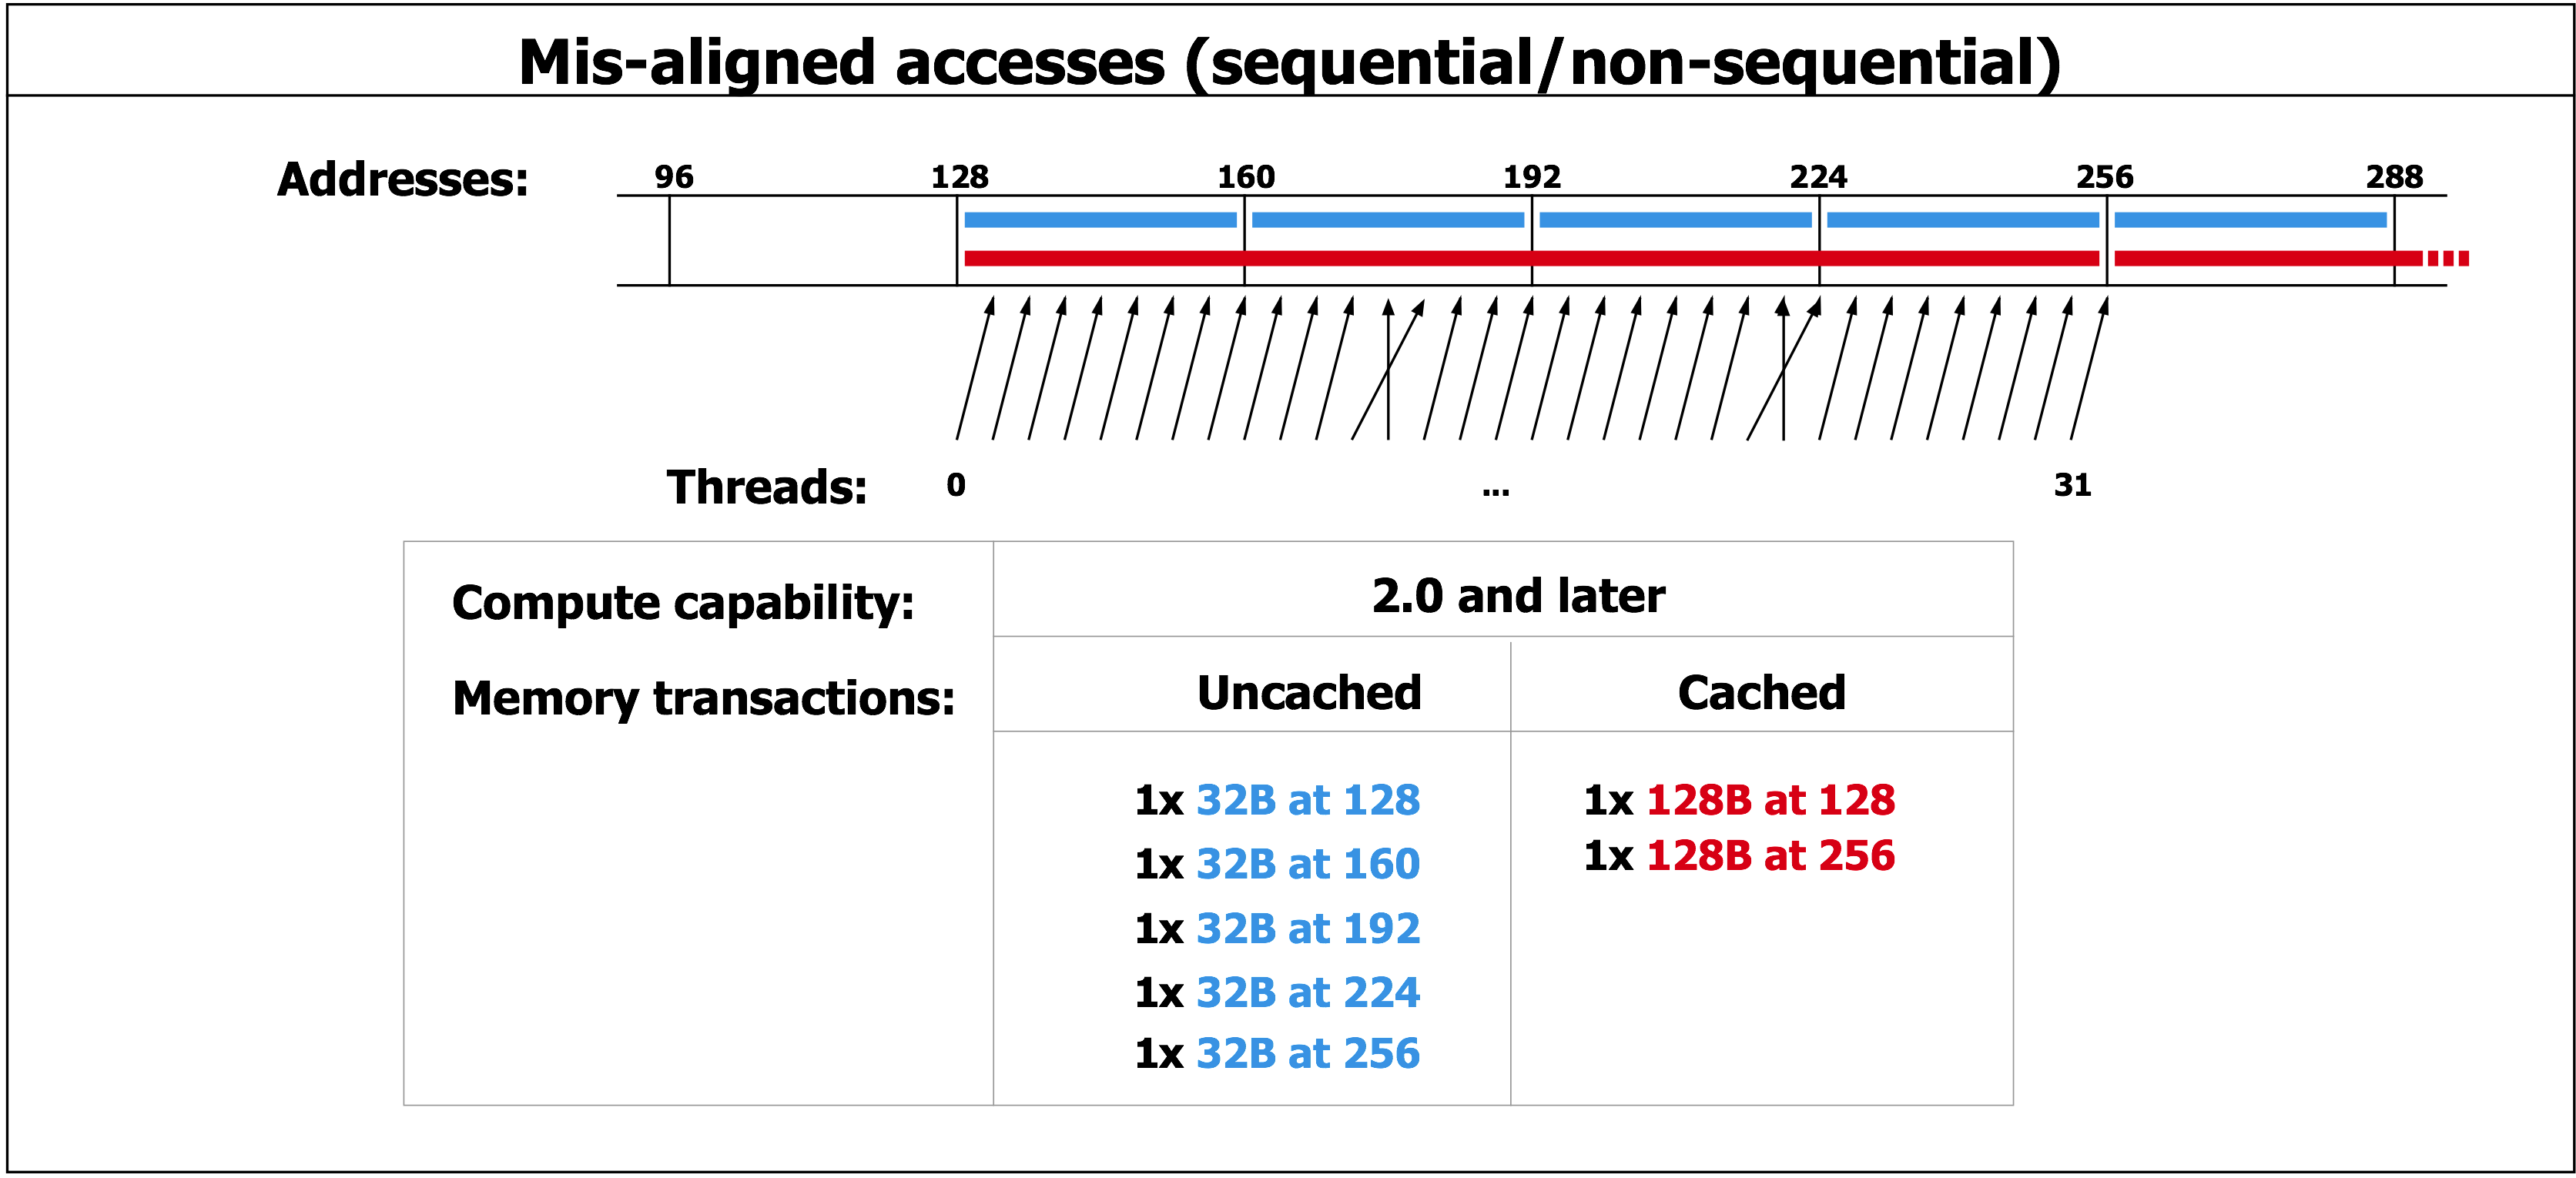
\includegraphics[height=0.3\textheight]{coa2}
	\end{figure}
}

\begin{document}

\frame
{
	\titlepage
}

\frame
{
	\frametitle{Overview}
		\begin{enumerate}
		\item CUDA Compilation
		\item PTX and Shader Assembly
		\item Profiling with Nsight Compute
		\item Various Optimization Techniques
		\begin{itemize}
		\item Grid Stride Loops
		\item Global Memory Access Patterns
		\item Occupancy
		\item Pinned Memory
		\item Streams + Parallel Kernels
		\end{itemize}
		\end{enumerate}
}

\frame
{
\begin{center}
\Large CUDA Compilation
\end{center}
}


\frame
{
	\frametitle{CUDA Compilation}
		\begin{figure}
	\centering
	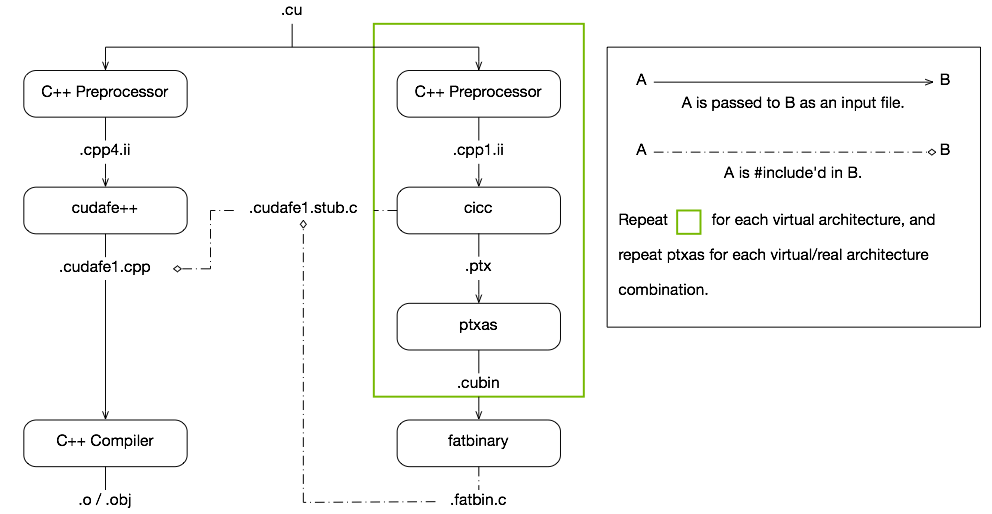
\includegraphics[height=0.95\textheight]{nvcc}
\end{figure}
}


\begin{frame}[fragile]
	\frametitle{Nvidia C Compiler (nvcc)}
	\begin{itemize}
		\item Supports C and C++
		\item Splits source files into host and device code
		\item Compiles device code to PTX and SASS
		\item Embeds the compiled device code in a synthetic C++ file
		\item Passes the generated C++ file to the host compiler (for example gcc)
	\end{itemize}	
Compiling a single source file into an executable named \textit{main}:
\begin{lstlisting}[language=bash]
nvcc -arch=sm_61 -g main.cu -o main
\end{lstlisting}
\end{frame}



\begin{frame}[fragile]
\frametitle{nvcc compiler flags}

\begin{itemize}
	
	\item[] \textbf{-g}
	\begin{itemize}
		\item[] Generate debug information for host code.
	\end{itemize}
	
		\item[] \textbf{-G}
	\begin{itemize}
		\item[] Generate debug information for device code. Turns off all optimizations. 
	\end{itemize}

	\item[] \textbf{-lineinfo}
\begin{itemize}
	\item[] Generate line-number information for device code.
\end{itemize}

\item[] \textbf{-src-in-ptx}
\begin{itemize}
	\item[] Interleave source in PTX. May only be used in conjunction with -G or -lineinfo. 
\end{itemize}

	\item[] \textbf{-ptx}
\begin{itemize}
	\item[] Compile all .cu input files to device-only .ptx files. This step discards the host code for each .cu input file. 
\end{itemize}

	\item[] \textbf{-V}
\begin{itemize}
	\item[]  	Print version information on this tool.
\end{itemize}

\end{itemize}
\end{frame}


\begin{frame}[fragile]
\frametitle{nvcc compiler flags}

\begin{itemize}
\item[] \textbf{-Xcompiler=[flag]}
\begin{itemize}
\item[] Passes [flag] to the CUDA host compiler
\end{itemize}

\item[] \textbf{--expt-relaxed-constexpr}
\begin{itemize}
\item[] Allows constexpr functions without \texttt{device} keyword to be used in device code
\end{itemize}

\item[] \textbf{--relocatable-device-code=true}
\begin{itemize}
\item[] Required for dynamic parallelism
\end{itemize}

\item[] \textbf{-restric}
\begin{itemize}
\item[] Assert that all kernel pointer parameters are restrict pointers.
\end{itemize}

\item[] \textbf{--profile}
\begin{itemize}
\item[] Instrument generated code/executable for use by gprof.
\end{itemize}


\end{itemize}
\end{frame}


\begin{frame}[fragile]
\frametitle{nvcc compiler flags}

\begin{itemize}
	\item[] \textbf{-arch}
	\begin{itemize}
		\item[] Specify the name of the class of NVIDIA virtual GPU architecture for which the CUDA input files must be compiled. 
	\end{itemize}
	
	\item[] \textbf{-code}
	\begin{itemize}
		\item[] Specify the name of the NVIDIA GPU to assemble and optimize PTX for. 
	\end{itemize}
	
	\item[] \textbf{-maxrregcount}
	\begin{itemize}
		\item[] Specify the maximum amount of registers that GPU functions can use. 
	\end{itemize}

	\item[] \textbf{-use\_fast\_math}
\begin{itemize}
	\item[] Make use of fast math library.
\end{itemize}


\item[] \textbf{-res-usage}
\begin{itemize}
	\item[] Show resource usage such as registers and memory of the GPU code. 
\end{itemize}

\end{itemize}
\end{frame}



\begin{frame}[fragile]
\frametitle{CUDA Compile Architectures}
	
		\begin{tabular}{c|l|l|l}
		Architecture & virtual arch flag & code flag & Graphic Cards\\	
		\hline
		Kepler & compute\_30 & sm\_30 & Geforce 700 Series\\
		Maxwell & compute\_52 & sm\_52 & Geforce 900 Series\\
		Pascal & compute\_61 & sm\_61 & Geforce 1000 Series\\
		Volta & compute\_70 & sm\_70 & Titan-V\\
		Turing & compute\_75 & sm\_75 & RTX 2000 Series\\	
	    Ampere & compute\_80 & sm\_80 & RTX 3000 Series\\	
	\end{tabular}
\\
	\vspace{0.6cm}
	Example command to compile for GTX 900 and 1000 Series:
\begin{lstlisting}[language=bash]
nvcc -gencode=arch=compute_52,code=sm_52 -gencode=arch=compute_61,code=sm_61 main.cu -o main
\end{lstlisting}
\end{frame}


\begin{frame}[fragile]
\frametitle{Just in time compilation (JIT)}
The PTX code for a virtual architecture can be embedded in a binary CUDA file. This will execute \texttt{ptxas} \textbf{at startup time} to compile the code for the current hardware. This has the following advantages/disadvantages:
\begin{itemize}
	\item Compiling is faster
	\item Starting the application takes longer
	\item Better compatibility to  different hardware
\end{itemize}
JIT can be enabled by repeating the virtual arch flag in the \texttt{code} flag:
\begin{lstlisting}[language=bash]
nvcc -gencode=arch=compute_30,code=compute_30 -gencode=arch=compute_61,code=sm_61 main.cu -o main
\end{lstlisting}
This example uses JIT for all architectures except sm\_61, because we told the compiler to generate SASS code for sm\_61.
\end{frame}

\begin{frame}[fragile]
\frametitle{NVCC and CMake}
\begin{itemize}
	\item The CUDA architecture is set by a target property
\end{itemize}
\begin{lstlisting}[language=bash]
set_property(TARGET hello_world PROPERTY 
	CUDA_ARCHITECTURES 52-virtual 61 70 80 )
\end{lstlisting}
\begin{itemize}
	\item Additional flags are appended to \texttt{CMAKE\_CUDA\_FLAGS} 
\end{itemize}
\begin{lstlisting}[language=bash]
list(APPEND MY_CUDA_FLAGS "-use_fast_math")
list(APPEND MY_CUDA_FLAGS "--expt-relaxed-constexpr")
list(APPEND MY_CUDA_FLAGS "-Xcompiler=-fopenmp")
list(APPEND MY_CUDA_FLAGS "-G")

# Add flags only to .cu files of the given target
target_compile_options(hello_world PRIVATE
  $<$<COMPILE_LANGUAGE:CUDA>:${MY_CUDA_FLAGS}>)
\end{lstlisting}

\end{frame}


\frame
{
\begin{center}
\Large PTX and SASS
\end{center}
}

\begin{frame}[fragile]
\frametitle{Parallel Thread Execution (PTX) ISA}
\begin{itemize}
	\item PTX is a low-level parallel thread execution virtual machine and instruction set architecture (ISA)
	\item Provides a stable ISA that spans multiple GPU generations.
	\item CUDA Device code is compiled to ptx and then from ptx to assembly
	\item \href{https://docs.nvidia.com/cuda/parallel-thread-execution/index.html}{PTX Documentation}
\end{itemize}
\textbf{Example \texttt{a[i] = b[i] + c[i]}:}
\begin{lstlisting}[language=bash]
add.s64 %rd8, %rd6, %rd7;
ld.global.f32 %f1, [%rd8];
add.s64 %rd9, %rd5, %rd7;
ld.global.f32 %f2, [%rd9];
add.f32 %f3, %f1, %f2;
add.s64 %rd10, %rd4, %rd7;
st.global.f32 [%rd10], %f3;
\end{lstlisting}
\end{frame}


\begin{frame}[fragile]
\frametitle{Shader Assembly (SASS)}
\begin{itemize}
\item SASS is the code executed by a specific GPU
\item Mostly similar to PTX, but
\begin{itemize}
	\item SASS is harder to read
	\item the documentation on SASS is a lot worse
\end{itemize}
\item \href{https://docs.nvidia.com/cuda/cuda-binary-utilities/index.html#maxwell-pascal}{Pascal Instruction Set reference}
\end{itemize}
\textbf{Example \texttt{a[i] = b[i] + c[i]}:}
\begin{lstlisting}[language=bash]
ISCADD R4.CC, R0, c[0x0][0x150], 0x2;
LD.E R2, [R2];              
IMAD.HI.X R5, R0, R7, c[0x0][0x154]; 
LD.E R4, [R4];            
ISCADD R6.CC, R0, c[0x0][0x140], 0x2; 
IMAD.HI.X R7, R0, R7, c[0x0][0x144];  
FADD R0, R2, R4; 
ST.E [R6], R0;    
\end{lstlisting}
\end{frame}


\begin{frame}[fragile]
	\frametitle{cuobjdump}
	\textbf{cuobjdump} extracts information from CUDA binary files. The extracted information include:
\begin{lstlisting}[language=bash]
cuobjdump [options] <file>
\end{lstlisting}
Example:
\begin{lstlisting}[language=bash]
# Extract code
cuobjdump -ptx simple_particle > ptx.txt
cuobjdump -sass simple_particle > sass.txt
# Show all cubins and extract one
cuobjdump -lelf simple_particle
cuobjdump -xelf simple_particle.sm_75.cubin simple_particle
\end{lstlisting}
\url{https://docs.nvidia.com/cuda/cuda-binary-utilities/index.html#cuobjdump}
\end{frame}

\begin{frame}[fragile]
	\frametitle{nvidisasm}
nvdisasm extracts information from standalone cubin files and presents them in human readable format. 
\begin{lstlisting}[language=bash]
nvdisasm [options] <input cubin file>
\end{lstlisting}
Example:
\begin{lstlisting}[language=bash]
# Convert to text
nvdisasm -c simple_particle.sm_75.cubin > asm.txt
# Register usage
nvdisasm -c -plr simple_particle.sm_75.cubin > asm.txt
\end{lstlisting}
\url{https://docs.nvidia.com/cuda/cuda-binary-utilities/index.html#nvdisasm}
\end{frame}

\frame
{
\begin{center}
\Large Profiling
\end{center}
}


\begin{frame}[fragile]
\frametitle{Profiling Tools}
Legacy Tools (Kepler - Volta)
\begin{itemize}
	\item Nvidia Visual Profiler (NVVP)
	\item NVProf (command line profiler)
\end{itemize}
\hrulefill \\
New Tools (Volta and newer)
\begin{itemize}
	\item Nsight Compute
	\item Nsight System
\end{itemize}
\vspace{0.5cm}
Source: \href{https://docs.nvidia.com/cuda/profiler-users-guide/index.html#migrating-to-nsight-tools}{Programming Guide}
\end{frame}


\begin{frame}[fragile]
\frametitle{Profiling}
Profile only a single simulation step:

\begin{lstlisting}
#ifdef CUDA_PROFILING
static int steps = 0;
if(steps == 300) cudaProfilerStart();
#endif

// The actual simulation step
particleSystem->update();

#ifdef CUDA_PROFILING
if(steps++ == 300){
	cudaProfilerStop();
	parentWindow.close();
}
#endif

\end{lstlisting}
\end{frame}




\frame
{
	\frametitle{Nsight Compute}
		\begin{figure}
	\centering
	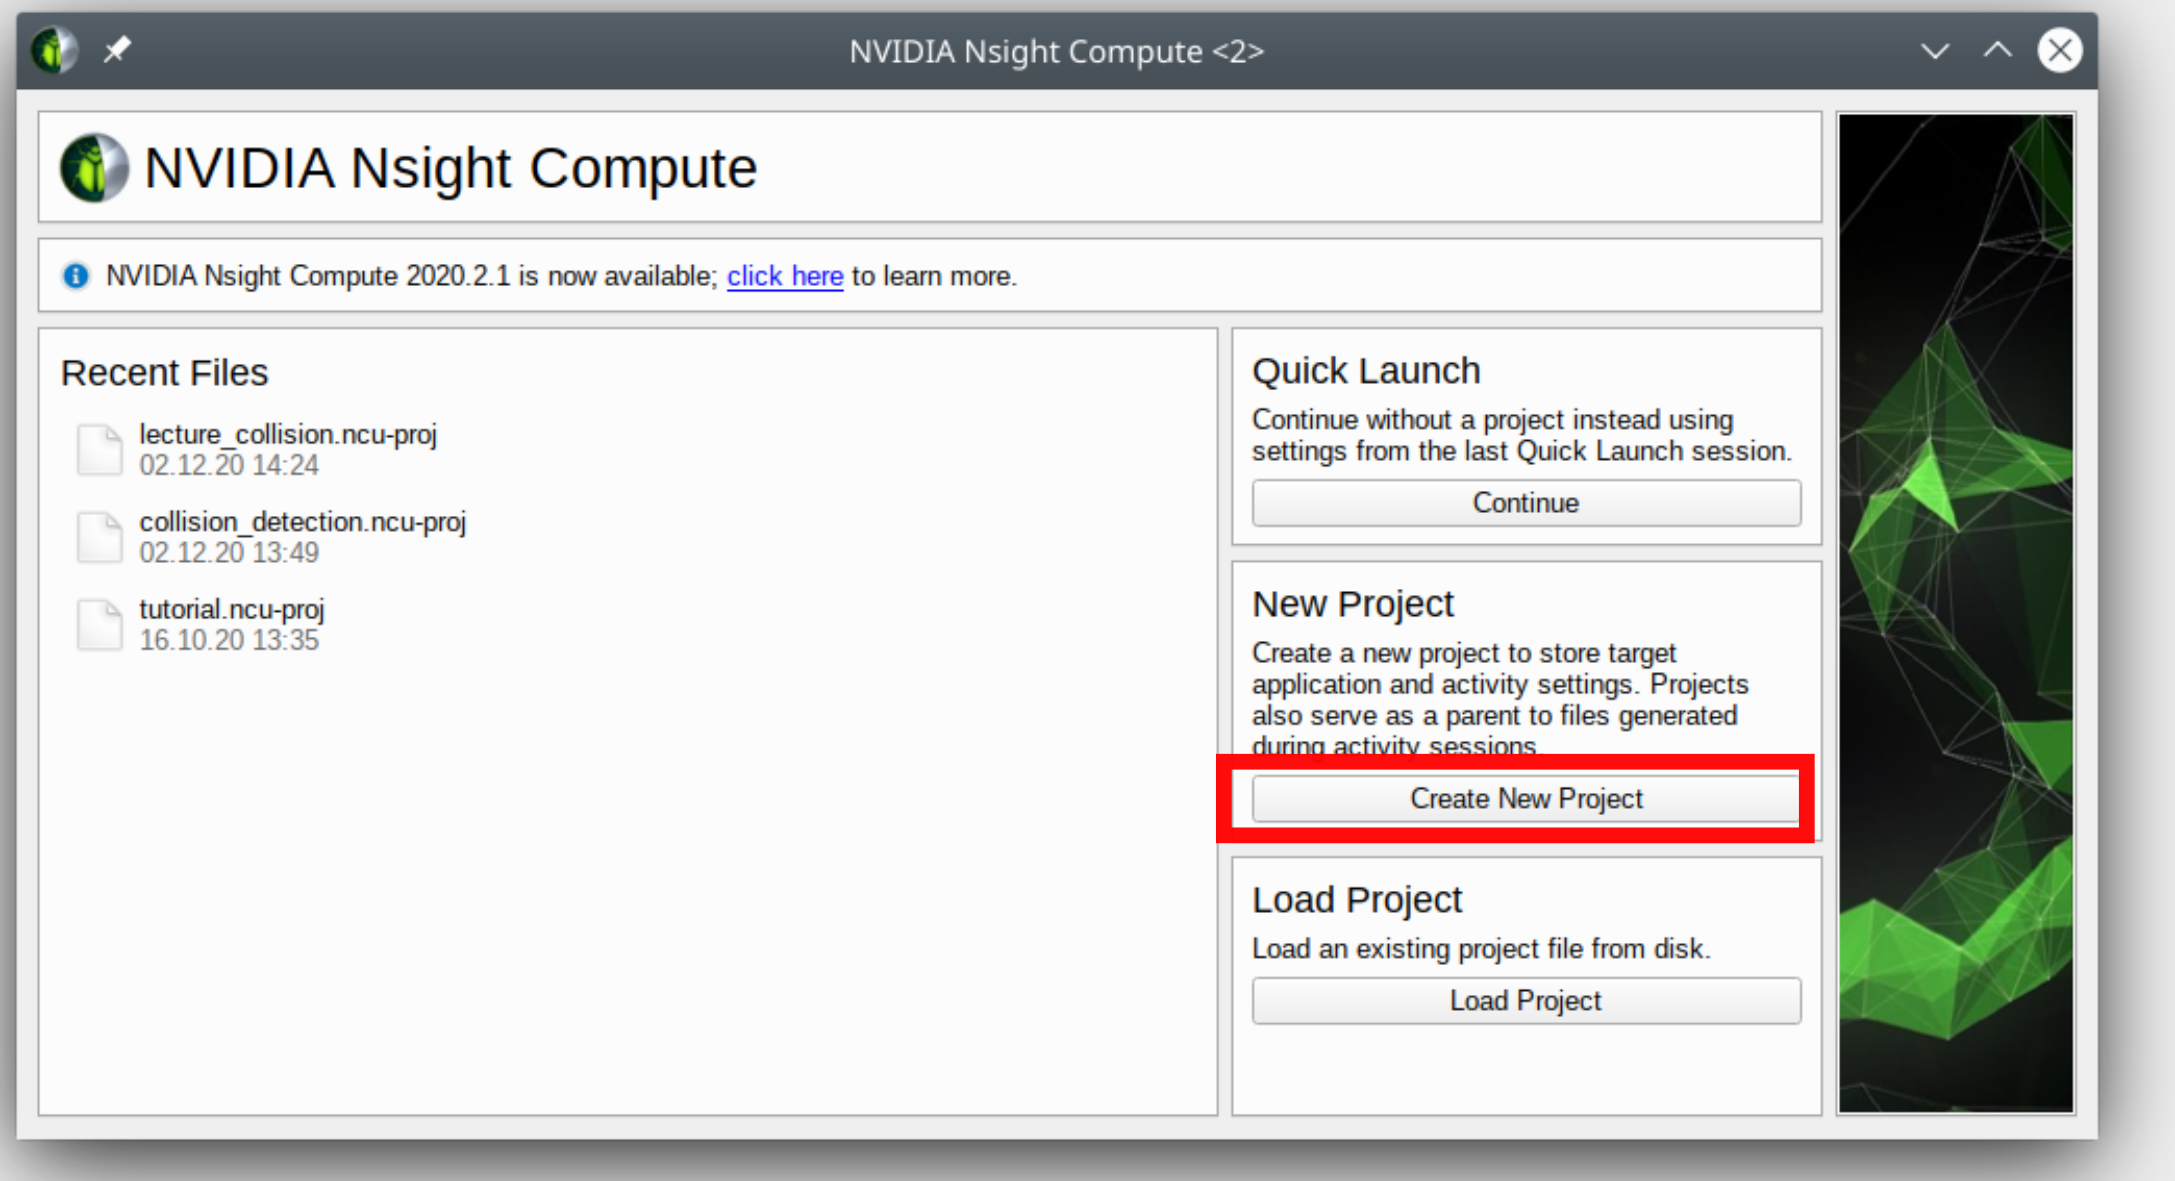
\includegraphics[height=0.95\textheight]{nsc1}
\end{figure}
}

\frame
{
	\frametitle{Nsight Compute}
		\begin{figure}
	\centering
	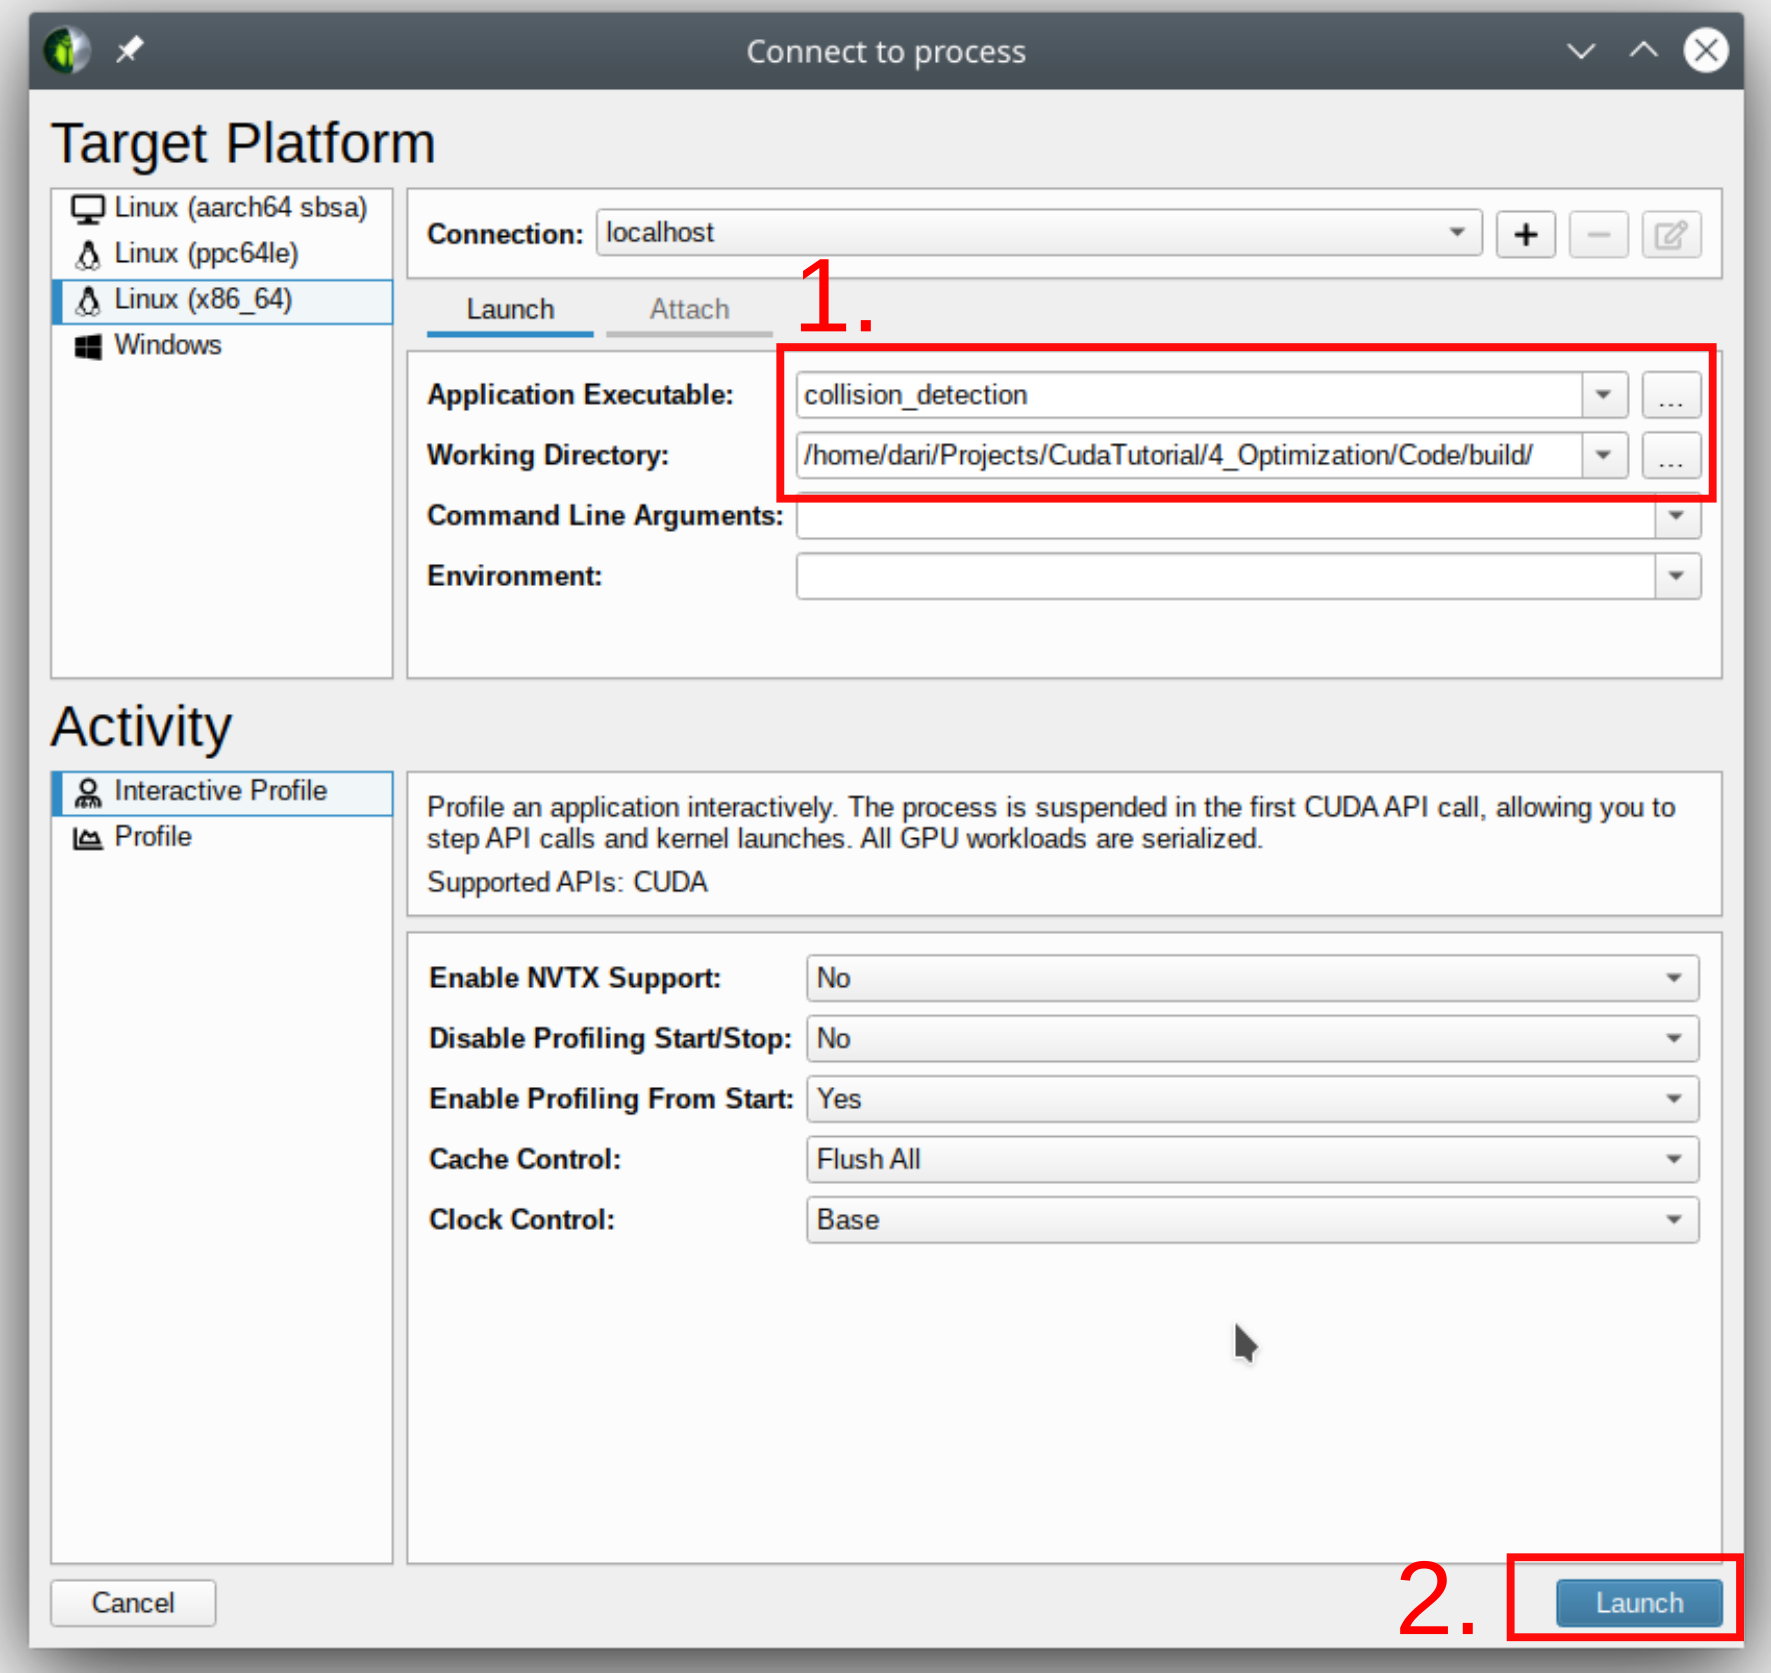
\includegraphics[height=0.95\textheight]{nsc2}
\end{figure}
}
\frame
{
	\frametitle{Nsight Compute}
		\begin{figure}
	\centering
	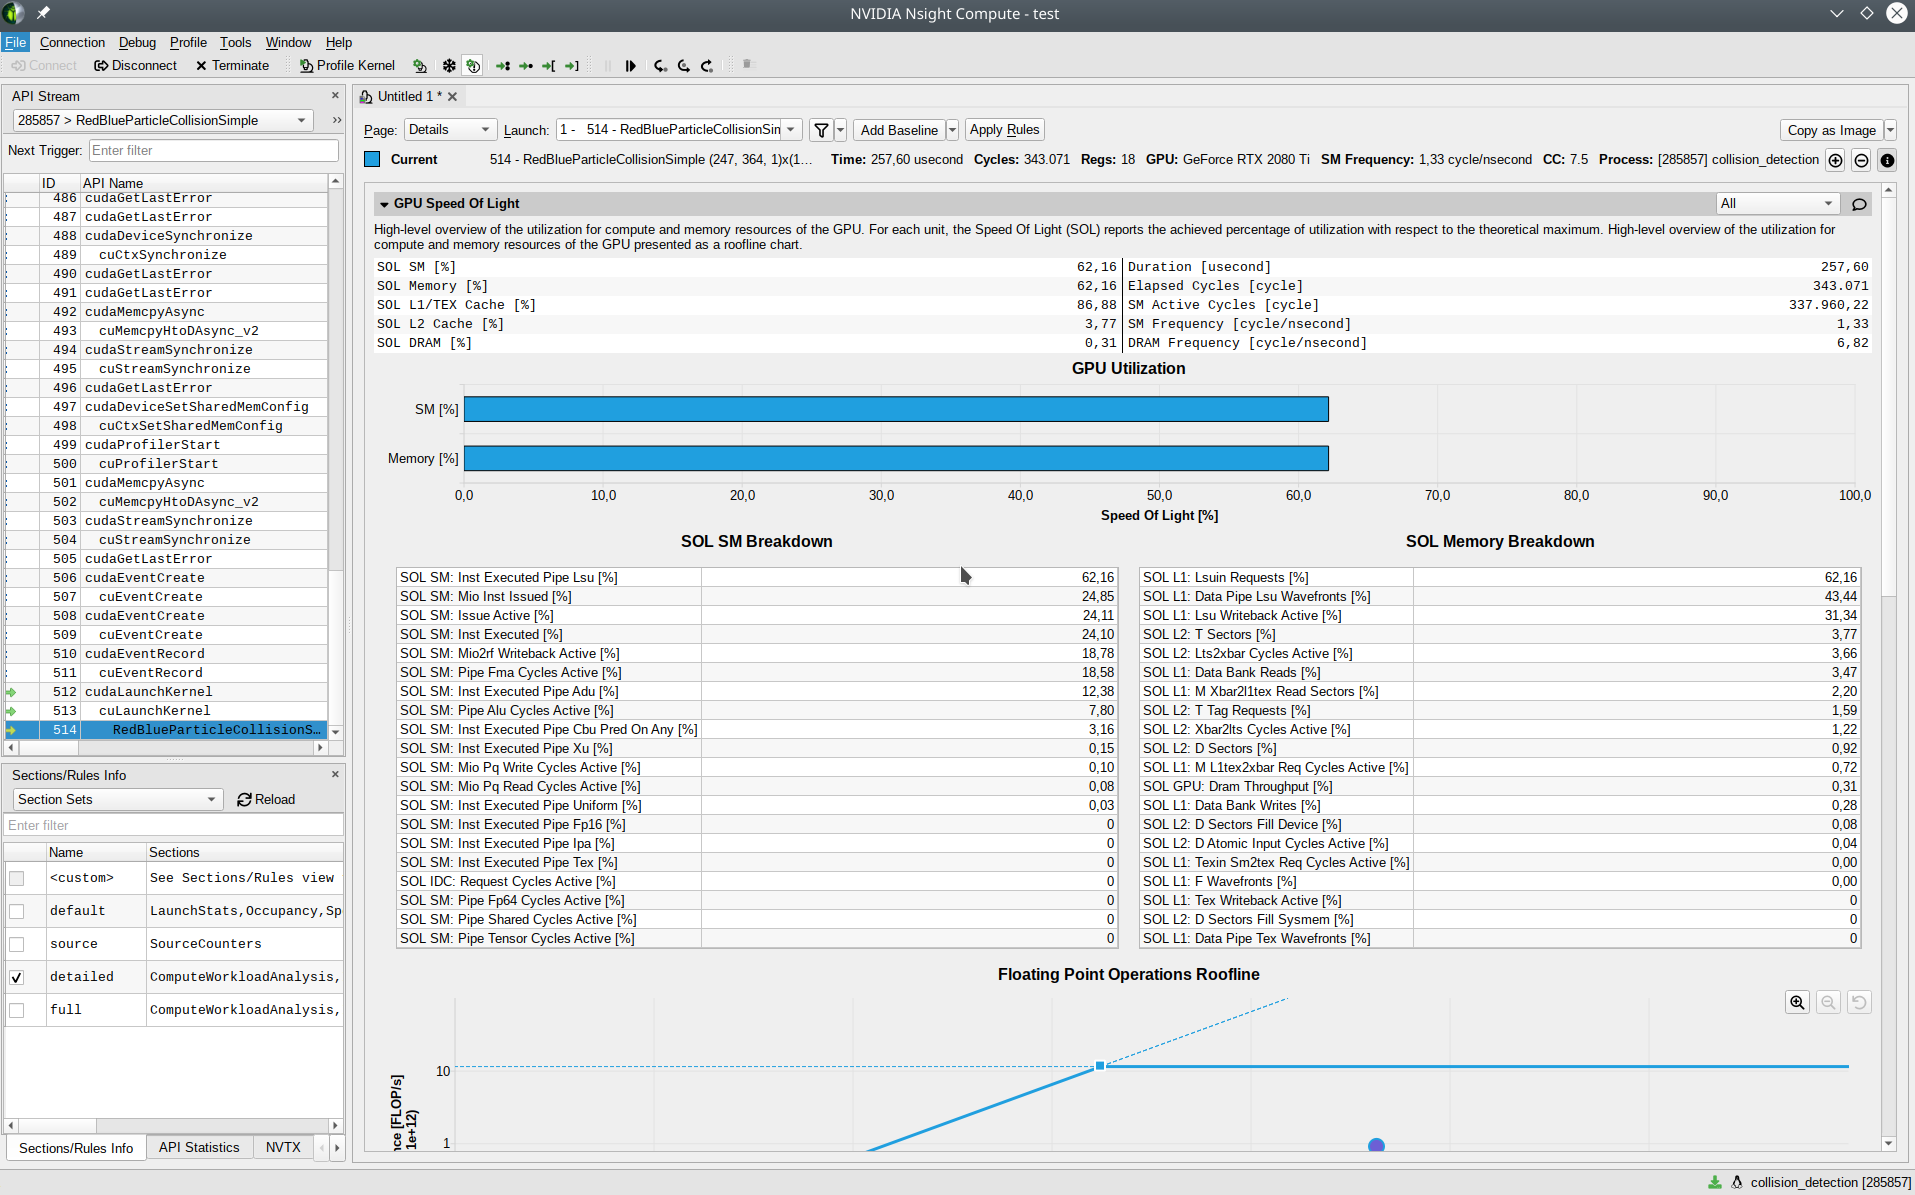
\includegraphics[height=0.95\textheight]{nsc3}
\end{figure}
}


\frame
{
\begin{center}
\Large Advanced Optimization Techniques
\end{center}
}


\begin{frame}[fragile]
\frametitle{Grid Stride Loops}

\begin{itemize}
\item Gride Stride Loops are a CUDA technique to make (linear) kernels more flexible
\item Gride Stride Loops improve
\begin{itemize}
\item Performance
\item Debugging
\item Portability
\end{itemize}
Source: \url{https://developer.nvidia.com/blog/cuda-pro-tip-write-flexible-kernels-grid-stride-loops/}
\end{itemize}
\end{frame}


\begin{frame}[fragile]
\frametitle{Grid Stride Loops}
Linear saxpy Kernel:
\begin{lstlisting}
__global__
void saxpy(int n, float a, float *x, float *y)
{
	int i = blockIdx.x * blockDim.x + threadIdx.x;
	if (i < n) 
	{
		y[i] = a * x[i] + y[i];
	}
}
\end{lstlisting}
\textbf{Note:} Every thread processes at most one element.
\end{frame}


\begin{frame}[fragile]
\frametitle{Grid Stride Loops}
saxpy Kernel with grid stride loop:
\begin{lstlisting}
__global__
void saxpy_gsl(int n, float a, float *x, float *y)
{
	int i = blockIdx.x * blockDim.x + threadIdx.x; 
	while(i < n)                     // Replace 'if' by 'while'
	{
		y[i] = a * x[i] + y[i];
		i += blockDim.x * gridDim.x;   // Increment by the grid size
	}
}
\end{lstlisting}
\textbf{Note:} This kernel can now be launched with an arbitrary grid- and block-size
\end{frame}




\begin{frame}[fragile]
\frametitle{Grid Stride Loops}
Without GS-Loop:
\begin{lstlisting}
saxpy<<< iDivUp(n,128),128 >>>(n, a, x, y);
\end{lstlisting}
With GS-Loop:
\begin{lstlisting}
// Launch 1 Block
saxpy_gsl<<< 1,128 >>>(n, a, x, y);
// Launch 1 Warp
saxpy_gsl<<< 1,32 >>>(n, a, x, y);
// Launch 1 Thread
saxpy_gsl<<< 1,1 >>>(n, a, x, y);
\end{lstlisting}
\begin{itemize}
	\item[$\rightarrow$] The kernel can be launched in any configuration
\end{itemize}
\end{frame}



\begin{frame}[fragile]
\frametitle{Grid Stride Loops}
\textbf{Debugging}
\begin{itemize}
\item Launching the kernel with 1 block or thread makes debugging easier
\item[$\rightarrow$] We can eliminate race conditions 
\item[$\rightarrow$] printf() and asserts are more meaningful
\end{itemize}

\textbf{Optimization}
\begin{itemize}
\item The number of launched blocks can now be tuned
\item For example, we can launch as many blocks as the GPU is able to run simultaneously 
\item[$\rightarrow$] Less blocks
\item[$\rightarrow$] Reduce scheduling cost
\end{itemize}
Grid Stride Loops are therefore used in many GPU libraries.
\end{frame}


\begin{frame}[fragile]
\frametitle{Pytorch Example}
\begin{itemize}
\item Index Select Kernel (ATen/native/cuda/indexing.cu):
\end{itemize}

\begin{lstlisting}
template <typename T, ...>
__global__ void indexSelect(
		cuda::detail::TensorInfo<T, IndexType> dst,
		...) 
{
	// Grid Stride loop
	for (IndexType linearIndex = blockIdx.x * blockDim.x + threadIdx.x;
	   linearIndex < totalSize;
	   linearIndex += gridDim.x * blockDim.x) {
	   // ...
	}
}
\end{lstlisting}
\end{frame}


\frame
{
\begin{center}
\Large Optimizing Global Memory Throughput
\end{center}
}


\begin{frame}[fragile]
\frametitle{Optimizing Global Memory Throughput}

\begin{mdframed}[frametitle={Cuda Programming Guide:}]
Optimizing the memory access pattern is especially important for global memory as the bandwidth is low compared to available on-chip bandwidths and arithmetic instruction throughput, so non-optimal global memory accesses generally have a high impact on performance. 
\end{mdframed}

\end{frame}


\begin{frame}[fragile]
\frametitle{Memory Access Overview}
\textbf{Optimization Checklist:}
\begin{enumerate}
	\item Align warp memory access to transaction size
	\item Reduce the number of load/store instructions
	\item Maximize coalescing in a warp
\end{enumerate}
\end{frame}


\begin{frame}[fragile]
\frametitle{Memory Checklist 1}
\begin{mdframed}[]
Align warp memory access to transaction size
\end{mdframed}
\vspace{0.3cm}
\begin{itemize}
\item The global memory is read and written using transactions
\item The transaction size is default 32B 
\item If the L1 cache is used the transactions are increased to 128B
\item Transactions are issued on a per-warp basis
\end{itemize}
\end{frame}

\begin{frame}[fragile]
\frametitle{Aligned Memory Accesses}
\begin{lstlisting}
int i = globalArray[threadIdx.x];
\end{lstlisting}
		\begin{figure}
		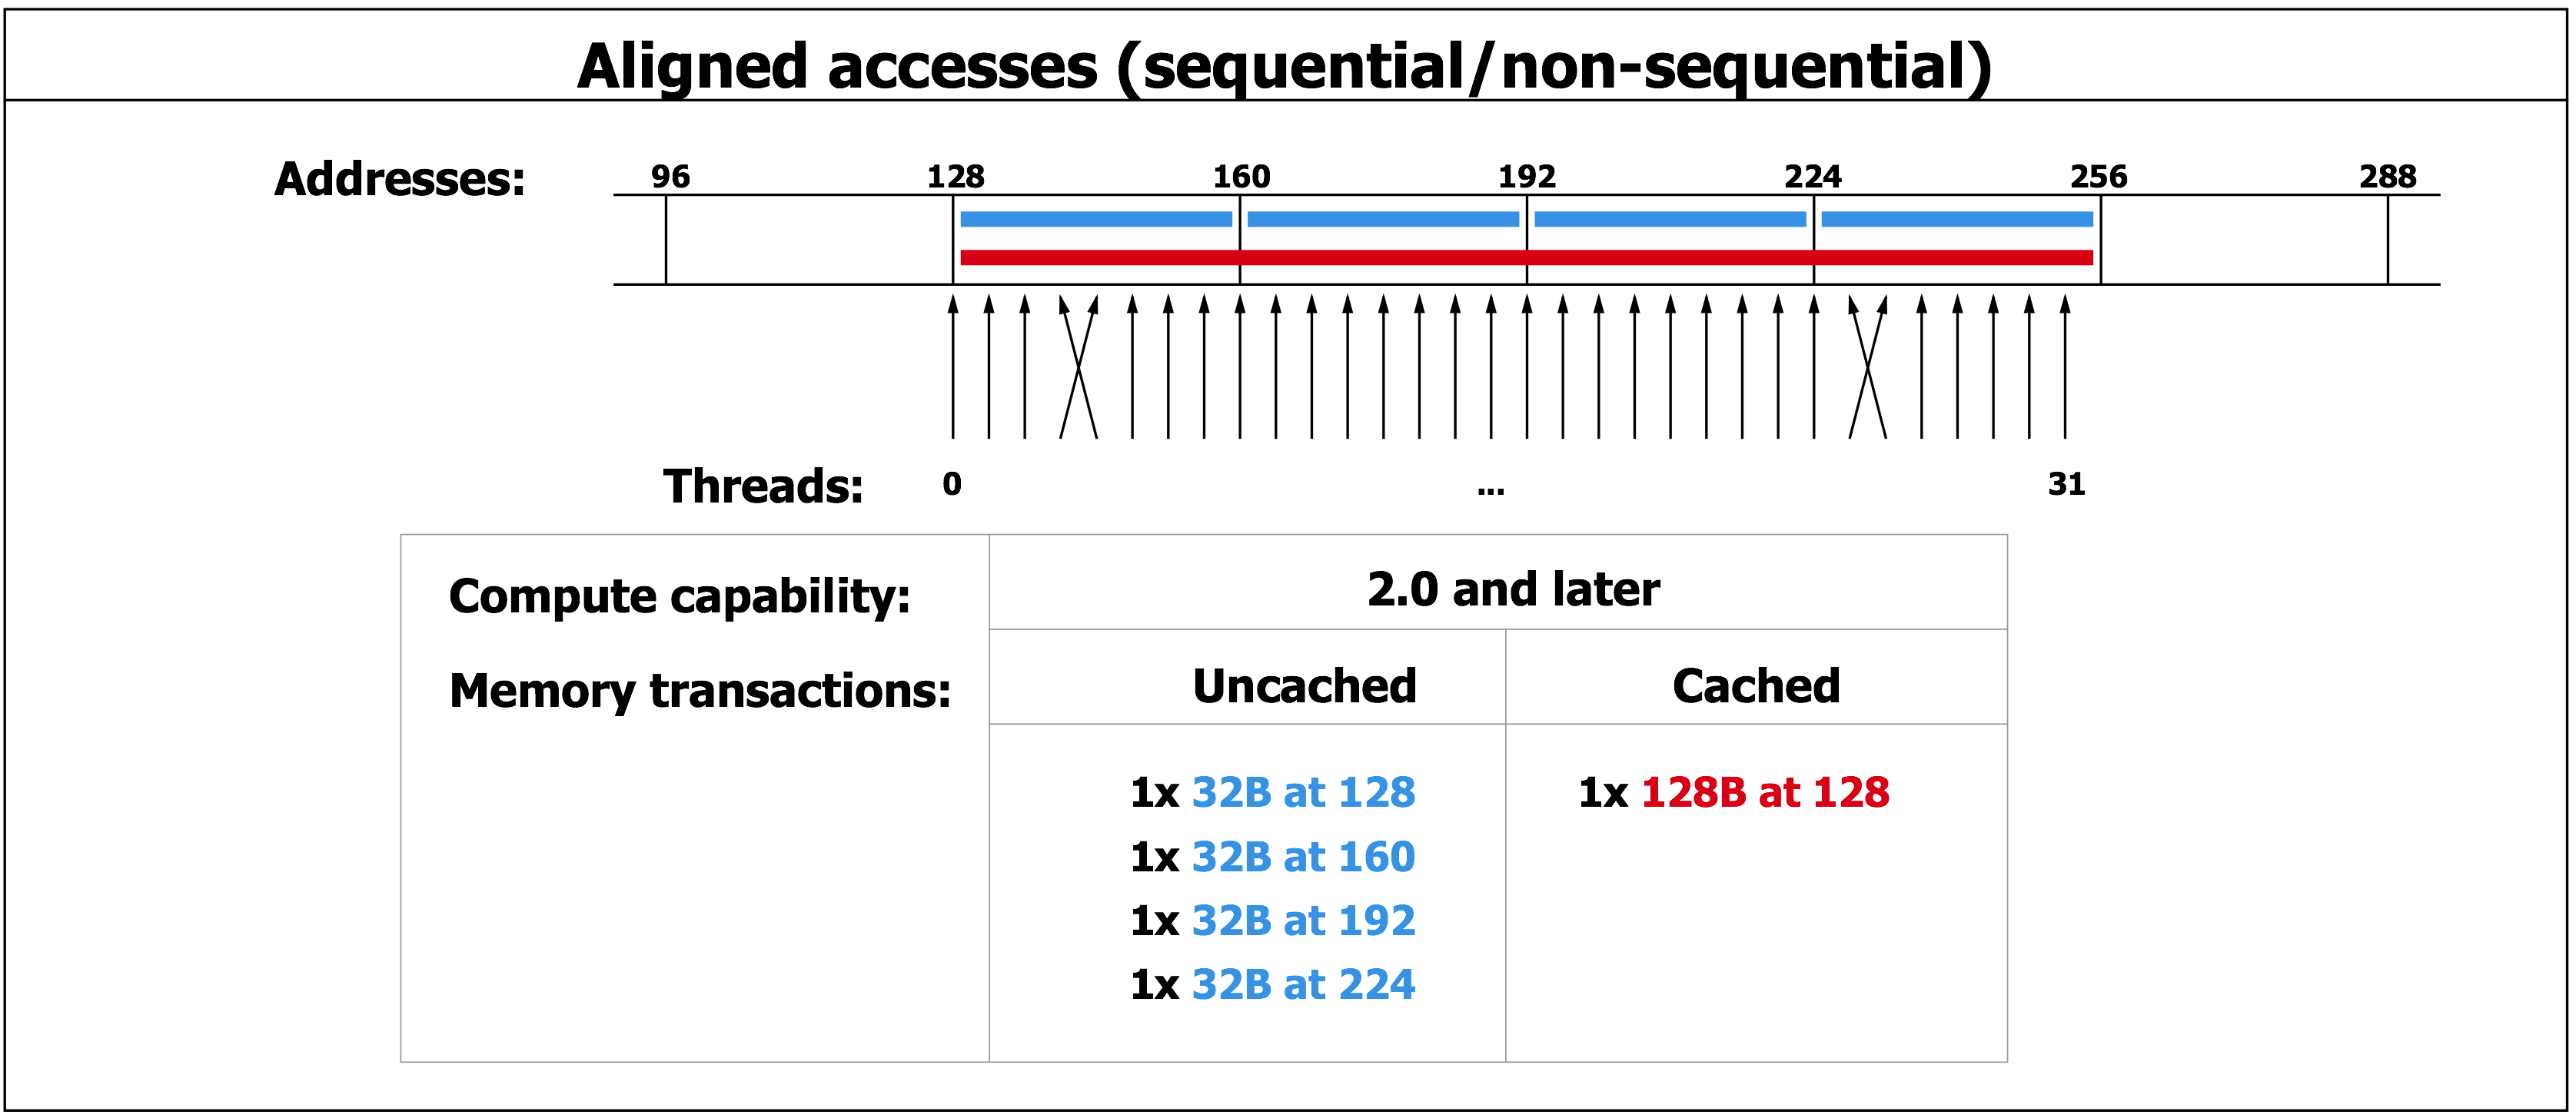
\includegraphics[height=0.7\textheight]{coa1}
	\end{figure}
\begin{itemize}
	\item[$\rightarrow$] 4 transactions per warp (uncached)
	\end{itemize}
\end{frame}

\begin{frame}[fragile]
	\frametitle{Misaligned Memory Accesses}
\begin{lstlisting}
int i = globalArray[threadIdx.x + 1];
\end{lstlisting}
		\begin{figure}
	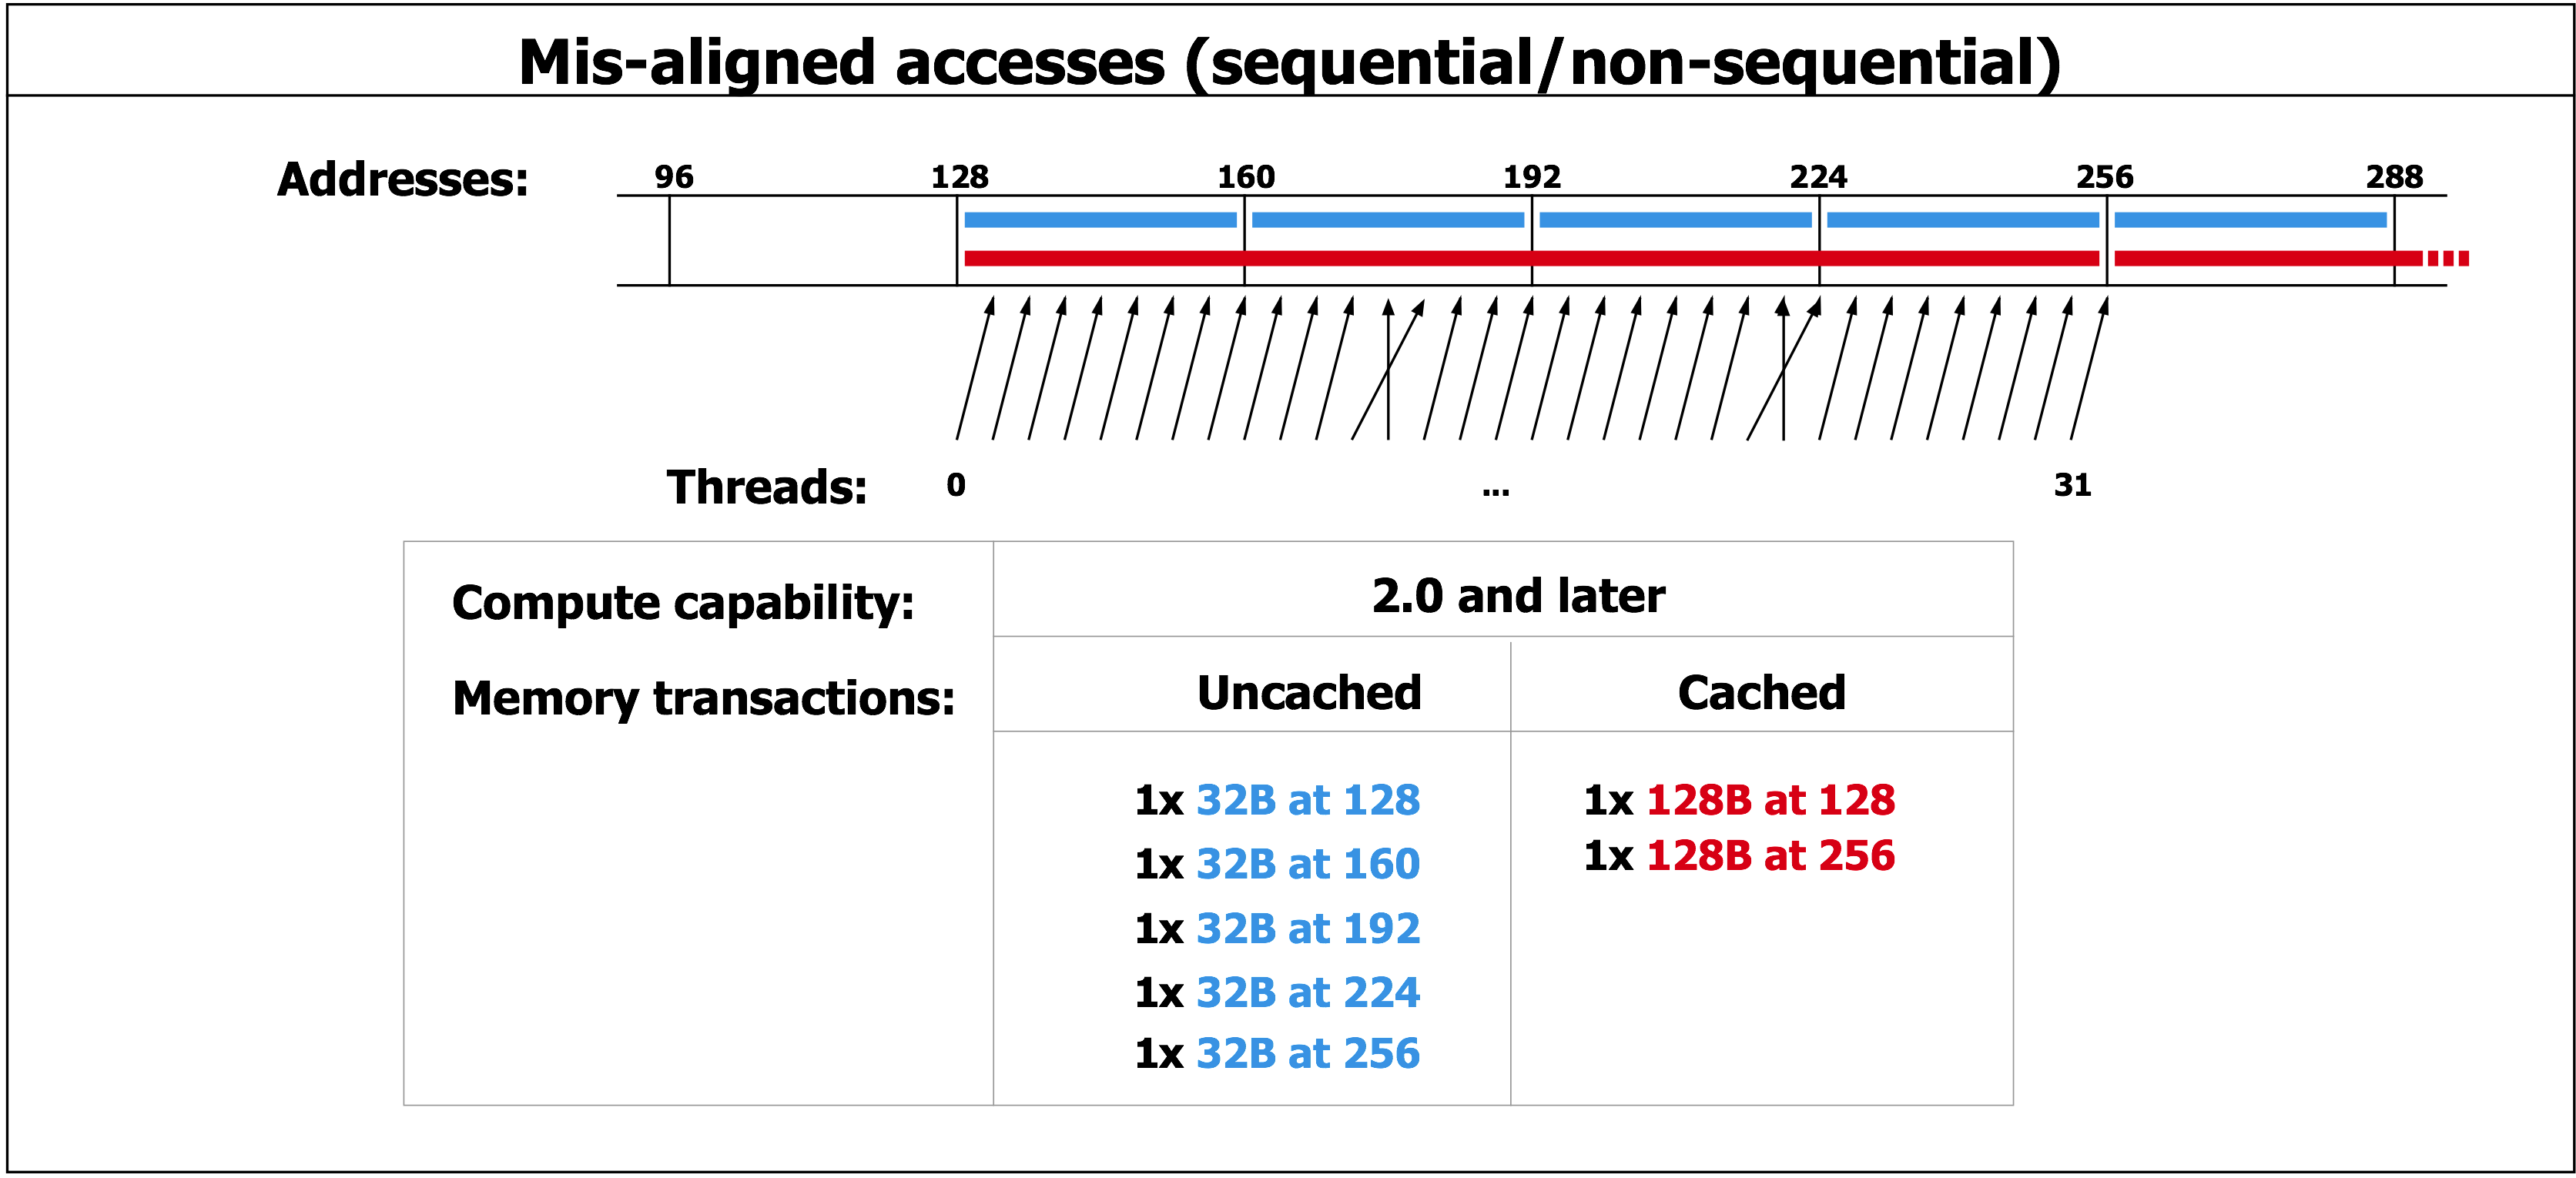
\includegraphics[height=0.7\textheight]{coa2}
\end{figure}
\begin{itemize}
	\item[$\rightarrow$] 5 transactions per warp (uncached), 25\% more than optimal
	\end{itemize}
\end{frame}


\begin{frame}[fragile]
\frametitle{Memory Checklist 2}
\begin{mdframed}[]
Reduce the number of load/store instructions
\end{mdframed}
\vspace{0.3cm}
The obvious answer
\begin{itemize}
\item Reduce C++ instructions that read/write global memory
\item Store values in registers/shared memory etc.
\end{itemize}
The less obvious answer
\begin{itemize}
\item Combine multiple load instructions into fewer, vectorized instructions
\item[$\rightarrow$] We can load up to 16 byte in a single instruction!
\end{itemize}
\end{frame}

\begin{frame}[fragile]
\frametitle{Vectorized Load Store}
\begin{itemize}
\item SASS provides load store instructions for 4, 8, and 16 byte global memory access:
\begin{itemize}
	\item \texttt{LD.E \ \ \ \ <dst reg>, <source address>}
	\item \texttt{LD.E.64 \ <dst reg>, <source address>}
	\item \texttt{LD.E.128 <dst reg>, <source address>}
\end{itemize}
\item They are always generated on the build-in types (int4, float2, ...)
\item Not always generated for custom structs with multiple members
\end{itemize}
\end{frame}

\begin{frame}[fragile]
	\frametitle{Vectorized Load Store (Bad)}
\begin{lstlisting}       
struct EIGEN_ALIGN16 Particle {
	vec3 position;
	float radius
};  
// ...
Particle p = particles[tid];
// ...
\end{lstlisting} 
Generated Code:
\begin{lstlisting}   
LD.E.64 R8,  [R4+0x4];                    
LD.E    R11, [R4+0x14];                  
LD.E    R7,  [R4+0xc];   
\end{lstlisting} 
\begin{itemize}
	\item[$\rightarrow$] 3 Load instructions instead of 1 even though the particle is aligned :c
\end{itemize}
\end{frame}


\begin{frame}[fragile]
	\frametitle{Vectorized Load Store (Good)}
	Force the compiler to generate a 16B load using a reinterpreting cast
\begin{lstlisting}       

// ...
Particle p;
reinterpret_cast<int4*>(&p)[0] = 
				reinterpret_cast<int4*>(particles + tid)[0];
// ...
\end{lstlisting} 
Generated Code:
\begin{lstlisting}   
LD.E.128 R8,  [R4+0x4];    
\end{lstlisting} 
\begin{itemize}
	\item[$\rightarrow$] Only 1 load instruction. This is now optimal.
\end{itemize}
\end{frame}


\begin{frame}[fragile]
\frametitle{Memory Checklist 3}
\begin{mdframed}[]
Maximize coalescing in a warp
\end{mdframed}
\vspace{0.3cm}
\begin{itemize}
\item Global memory read/writes of a warp are coalesced (combined) into a few transactions
\item We want to reduce the number of transactions
\item[$\rightarrow$] Neighboring threads should access neighboring (or the same) elements
\item[$\rightarrow$] Strided memory access reduces performance
\end{itemize}
\end{frame}

\begin{frame}[fragile]
	\frametitle{Strided Access 1}
	\begin{itemize}
	\item The read/written element is smaller than the gap between those elements
	\item Naturally occurs by accessing members of a struct
\end{itemize}
Example:
\begin{lstlisting}       
struct EIGEN_ALIGN32 Particle {
	float4 position;
	float4 velocity;
};  
// ...
float4 p = particles[tid].position;
float4 v = particles[tid].velocity;
// ...
\end{lstlisting} 
\end{frame}


\begin{frame}[fragile]
	\frametitle{Strided Access 2}
	\begin{itemize}
	\item 	\textbf{Non-coalescable memory access pattern}
\end{itemize}
	\begin{figure}
		\centering
		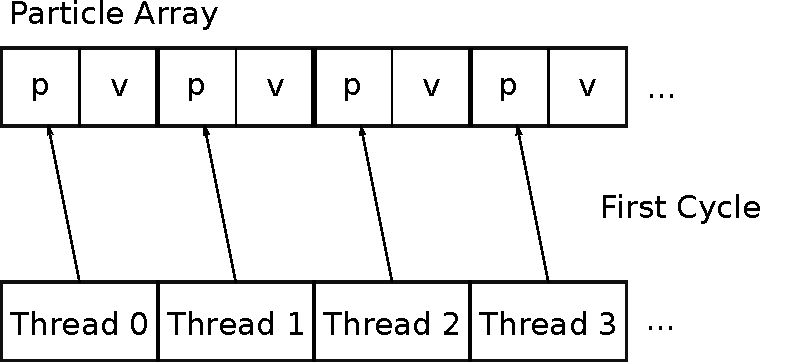
\includegraphics[height=0.5\textheight]{accessParticle1}
	\end{figure}
\begin{lstlisting}             
float4 p = particles[tid].position;
\end{lstlisting} 
\end{frame}


\begin{frame}[fragile]
	\frametitle{Strided Access 3}
	\begin{itemize}
		\item 	\textbf{Non-coalescable memory access pattern}
	\end{itemize}

	\begin{figure}
		\centering
		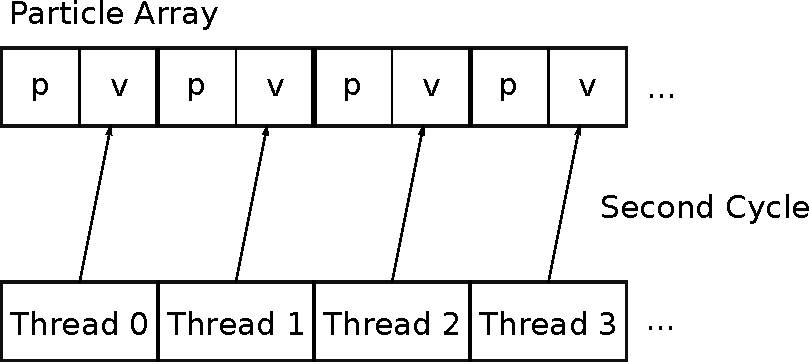
\includegraphics[height=0.5\textheight]{accessParticle2}
	\end{figure}
\begin{lstlisting}             
float4 v = particles[tid].velocity;
\end{lstlisting} 
\begin{itemize}
	\item[$\rightarrow$] 2 times more transactions than optimal
	\end{itemize}
\end{frame}

\begin{frame}[fragile]
\frametitle{Strided Access Solution}
Instead of storing and array of particles, we split it into
\begin{itemize}
	\item an array of positions
	\item an array of velocities
\end{itemize}
This concept is often called \textbf{structure of arrays} and is widely used in high performance computing and GPU libraries.
\begin{lstlisting}
vec4* positions = ...;
vec4* velocities = ...;
// ...
vec4 p = positions[tid];
vec4 v = velocities[tid];
// ...
\end{lstlisting}
\end{frame}



\begin{frame}[fragile]
\frametitle{Particle Integration Performance}
	\begin{tabular}{l|l|l|l}
	\textbf{Method} & \textbf{Time (ms)} & \textbf{Bandwidth (GB/s)} & \textbf{Speed Up} \\	
	\hline
	Initial & 0.458  & 139.509 & 1 \\
	Vector + Inverse Layout & 0.273  &       233.918 & 1.68 \\
	cudaMemcpy & 0.275   &    232.342 & 1.68  
\end{tabular}
\\
\vspace{0.5cm}
\begin{itemize}
	\item[$\rightarrow$] Optimizing the global memory access improves performance by around 68\%
	\item[$\rightarrow$] We have reached bandwidth limit (same BW as cudaMemcpy)
	\item[$\rightarrow$] \href{https://github.com/darglein/saiga/blob/master/samples/cuda/globalMemory/main.cu}{Full source code @ GitHub}
\end{itemize}
\end{frame}


\frame
{
\begin{center}
\Large Occupancy and Latency
\end{center}
}


\begin{frame}[fragile]
\frametitle{Occupancy}

%https://docs.nvidia.com/gameworks/content/developertools/desktop/analysis/report/cudaexperiments/kernellevel/achievedoccupancy.htm
	\begin{mdframed}[frametitle={CUDA Programming Guide}]
A warp is considered active from the time its threads begin executing to the time when all threads in the warp have exited from the kernel. There is a maximum number of warps which can be concurrently active on a Streaming Multiprocessor (SM). \textbf{Occupancy is defined as the ratio of active warps on an SM to the maximum number of active warps supported by the SM.}
\end{mdframed}
\end{frame}


\begin{frame}[fragile]
\frametitle{Occupancy Limiting Factors}
\textbf{Warps per SM}
\begin{itemize}
	\item The SM has a maximum number of warps that can be active at once. 
	\item For most current GPUs this limit is 64 (=2048 Threads)
\end{itemize}

\textbf{Blocks per SM}
\begin{itemize}
	\item The SM has a maximum number of blocks that can be active at once.
	\item A typical limit is 32 blocks per SM $\rightarrow$ Minimum block size is 64 threads
\end{itemize}		
\end{frame}

\begin{frame}[fragile]
\frametitle{Occupancy Limiting Factors}
\textbf{Registers per SM}
\begin{itemize}
	\item The SM has a set of registers shared by all active threads.
	\item For most current GPUs this limit is 65536 (32 registers per active thread)
\end{itemize}

\textbf{Shared Memory per SM}
\begin{itemize}
	\item The SM has a fixed amount of shared memory shared by all active threads. 
	\item The L1 cache resides in shared memory
	\item For current GPUs the limit is 98304 bytes (12 $\times$ 4 byte per active thread)
\end{itemize}		
\end{frame}


\begin{frame}[fragile]
\frametitle{Occupancy}
When does occupancy \textbf{not} matter?
\begin{itemize}
	\item For bandwidth limited kernels
	\item For compute bound kernels
\end{itemize}

When does occupancy matter?
\begin{itemize}
	\item For latency bound kernels
\end{itemize}		
\end{frame}



\begin{frame}[fragile]
\frametitle{Latency}

Similar to CPU threads, active warps can be either \textbf{running}, \textbf{ready} or \textbf{blocked}.
\begin{itemize}
	\item A running warp executes commands until a blocking instruction
	\item A blocked warp waits for an event
	\item A ready warp waits until a running warp stops 
	\item A running warp is never stopped by the scheduler
\end{itemize}

	\begin{figure}
	\centering
	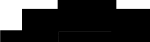
\includegraphics[height=0.3\textheight]{latency}
\end{figure}
\end{frame}


\begin{frame}[fragile]
\frametitle{Latency}

\begin{itemize}
	\item SMs on current GPUs can have 4 warps running at the same time
	\item Each SM can have 64 active warps
	\item[$\rightarrow$] With high occupancy, memory latency can be hidden by the scheduler
	\item[$\rightarrow$] With low occupancy, less than 3 warps might be running at the same time
\end{itemize}
\end{frame}



\begin{frame}[fragile]
\frametitle{Launch Bounds}
	The register usage can be controlled by the \texttt{\_\_launch\_bounds\_\_} intrinsic. \\
	\textbf{Syntax:}
\begin{lstlisting}
__launch_bounds__(MAX_THREADS_PER_BLOCK,MIN_BLOCKS_PER_SM)
\end{lstlisting}
\textbf{Example:}
\begin{lstlisting}
template<unsigned int BLOCK_SIZE>
__launch_bounds__(BLOCK_SIZE,MAX_THREADS_PER_SM/BLOCK_SIZE)
__global__ static
void collideParticlesLCK(...)
{
 	//...
}
\end{lstlisting}

\end{frame}



\frame
{
\begin{center}
\Large Pinned Memory
\end{center}
}



\begin{frame}[fragile]
\frametitle{Problem 1 - Paged Host Memory}
By default, all memory allocations on the Host are paged. A page table translates virtual page addresses to physical page addresses.
\begin{itemize}
	\item Memory can only be allocated in page-sized blocks
	\item Consecutive virtual pages can be fragmented in physical memory
	\item Pages can be swapped out
	\item Pageable memory cannot be used for DMA transfers
	\item[$\rightarrow$] Paged memory has to be copied to pinned/locked memory
\end{itemize}

\end{frame}



\begin{frame}[fragile]
\frametitle{Pinned Memory}

		\begin{figure}
	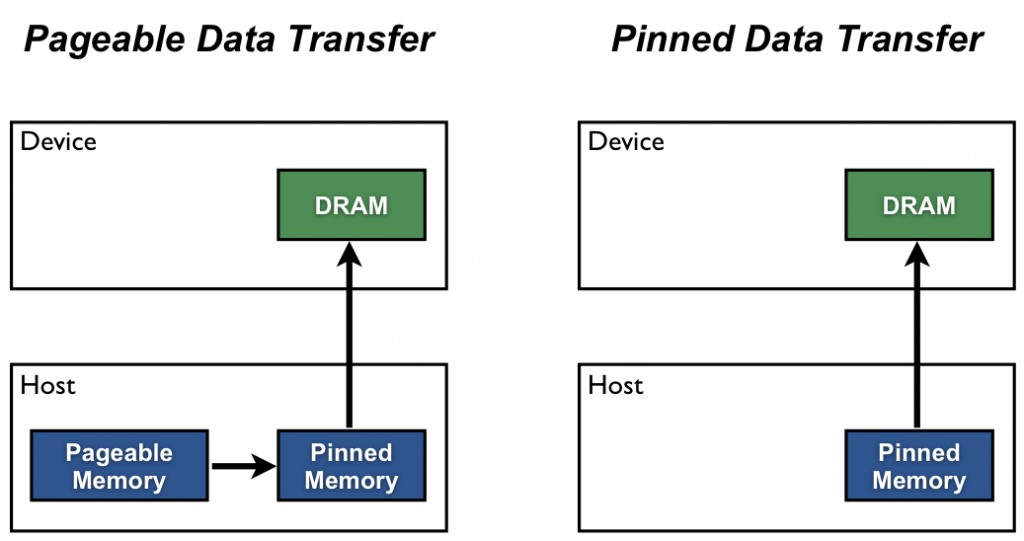
\includegraphics[height=0.7\textheight]{pinnend}
\end{figure}

\end{frame}


\begin{frame}[fragile]
\frametitle{Pinned Memory}
\begin{itemize}
	\item Pinned memory can be directly allocated and used
	\item Larger allocation overhead than pageable memory
	\item Limited by physical available host memory (no swapping)
\end{itemize}
Allocation with CUDA Runtime:
\begin{lstlisting}
int* h_data;
cudaMallocHost((void**)&h_data, N * sizeof(int));
\end{lstlisting}
Allocation with Saiga:
\begin{lstlisting}
#include "saiga/cuda/pinned_vector.h"
// ...

Saiga::thrust::pinned_vector<int> h_data(N);
\end{lstlisting}
\end{frame}



\frame
{
\begin{center}
\Large Streams
\end{center}
}



\frame
{
	\frametitle{GPU Concurrency}
	It is possible in CUDA to
	\begin{itemize}
		\item execute multiple kernels at the same time
		\item copy data while executing kernels
		\item copy data in both directions in parallel
	\end{itemize}
\onslide<2->
	But
	\begin{itemize}
		\item Non of these things are done by default
		\item[$\rightarrow$] The programmer has to control it explicitly via \textbf{Streams}
	\end{itemize}
}



\begin{frame}[fragile]
\frametitle{CUDA Streams}
	\begin{mdframed}[frametitle={CUDA Programming Guide}]
Applications manage the concurrent operations described above through streams. A stream is a sequence of commands (possibly issued by different host threads) that execute in order. Different streams, on the other hand, may execute their commands out of order with respect to one another or concurrently; this behavior is not guaranteed and should therefore not be relied upon for correctness (e.g., inter-kernel communication is undefined). 
\end{mdframed}
\end{frame}

\begin{frame}[fragile]
\frametitle{Creation and Destruction}

CUDA Runtime API
\begin{lstlisting}
cudaStream_t stream;
cudaStreamCreate(&stream);
cudaMemcpyAsync(dst,src,size,cudaMemcpyHostToDevice,stream);
cudaStreamDestroy(stream);
\end{lstlisting}

Saiga
\begin{lstlisting}
#include "saiga/cuda/stream.h"
//...

Saiga::CUDA::CudaStream stream;
cudaMemcpyAsync(dst,src,size,cudaMemcpyHostToDevice,stream);

// Destroyed in the destructor of 'stream'
\end{lstlisting}
\end{frame}

\begin{frame}[fragile]
\frametitle{Asynchronous memcpy}
\texttt{cudaMemcpy}
\begin{itemize}
	\item is synchronous
	\item[$\rightarrow$] the CPU waits until all kernels are finished
	\item[$\rightarrow$] the CPU waits until the data transfer is finished
\end{itemize}
\onslide<2->
\texttt{cudaMemcpyAsync}
\begin{itemize}
	\item<2-> is executed in-order for the given stream
	\item<3-> returns control immediately to the CPU
	\item<4-> only works with \textit{pinned} memory
	\item<5-> same syntax as \texttt{cudaMemcpy}
	\item<6-> Currently no Thrust wrapper
\end{itemize}
\end{frame}



\begin{frame}[fragile]
\frametitle{Explicit Synchronization}

\begin{itemize}
	\item Synchronize everything
	\begin{itemize}
		\item \texttt{cudaDeviceSynchronize}
		\item Blocks host until all issued CUDA calls are complete
	\end{itemize}
	\item Synchronize w.r.t. a specific stream
	\begin{itemize}
		\item \texttt{cudaStreamSynchronize(streamid)}
		\item Blocks host until all CUDA calls in streamid are complete
	\end{itemize}
	\item Synchronize using Events
	\begin{itemize}
		\item Create specific 'Events', within streams, to use for synchronization
		\item Streams can wait on each other without blocking the host
	\end{itemize}
\end{itemize}
\end{frame}


\begin{frame}[fragile]
\frametitle{CUDA Events}

\begin{itemize}
	\item Events are placed into command streams (record)
	\item Streams can wait for events of other streams
	\item In the next few slides the \href{https://github.com/darglein/saiga/blob/master/src/saiga/cuda/event.h}{CudaEvent c++ wrapper} from Saiga is used
	\item Example to measure GPU time with CudaEvents:
\end{itemize}
\begin{lstlisting}
CudaEvent start, stop;                           
start.record();                                  
// ...                                           
stop.record();                                   
stop.synchronize();                              
float time = CudaEvent::elapsedTime(start,stop); 
\end{lstlisting}
\end{frame}




\begin{frame}[fragile]
\frametitle{Concurrency Example}
Our Task:
\begin{enumerate}
	\item Copy array of elements to the GPU
	\item Process each element
	\item Copy array back to the CPU
\end{enumerate}
\end{frame}


\begin{frame}[fragile]
\frametitle{Optimization Idea}
\begin{itemize}
	\item Split the large array into multiple segments
	\item Interleave upload, process, and download
	\item Data is uploaded for a segment while the previous one is still processed
	\item[$\rightarrow$] Maximize concurrent GPU utilization
	\item[$\rightarrow$] Reduce the overall processing time
\end{itemize}
\end{frame}

\begin{frame}[fragile]
\frametitle{Interleaved transfer/process}

\begin{figure}
	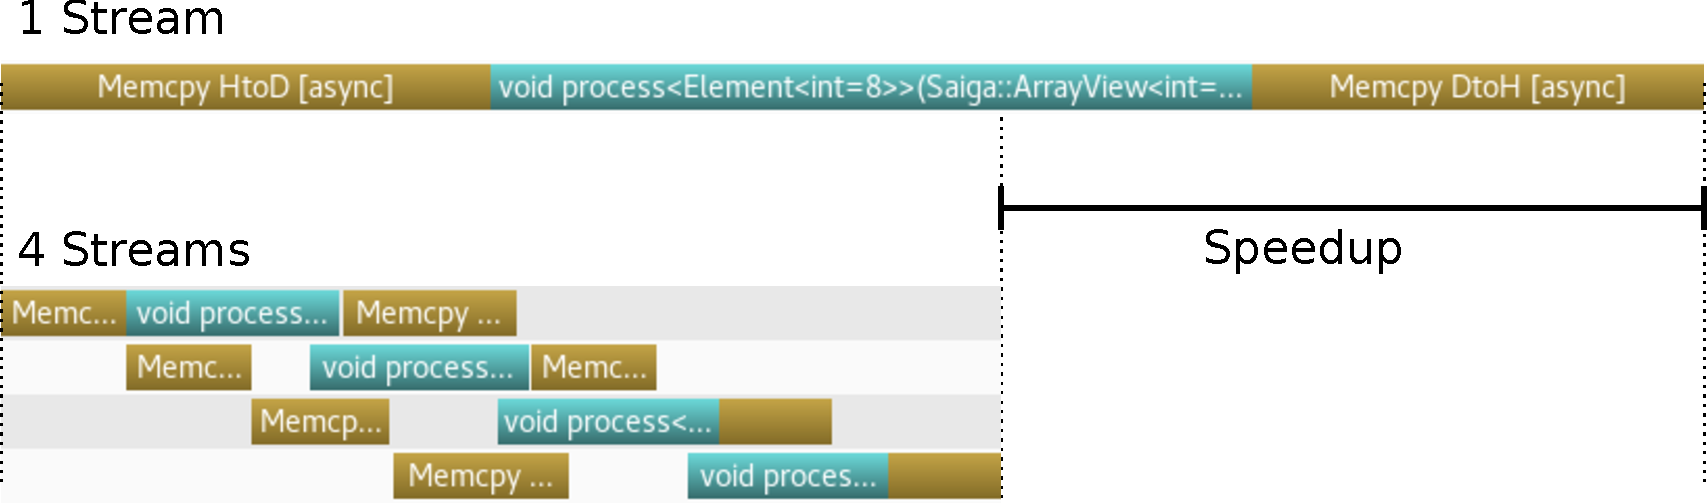
\includegraphics[width=1\linewidth]{asyncspeedup}
\end{figure}

\end{frame}

\begin{frame}[fragile]
\frametitle{Interleaved transfer/process}
16 Streams
\begin{figure}
	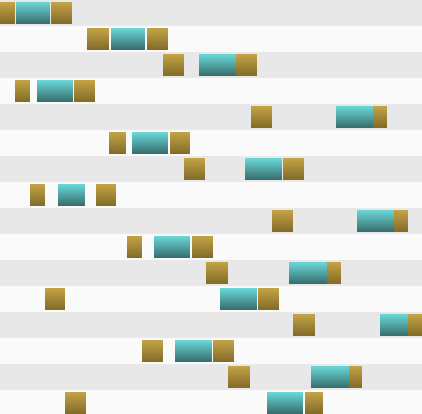
\includegraphics[width=.4\linewidth]{async16}
\end{figure}

\end{frame}

\begin{frame}[fragile]
\frametitle{Interleaved transfer/process}
8 Streams, 64 Slices
\begin{figure}
	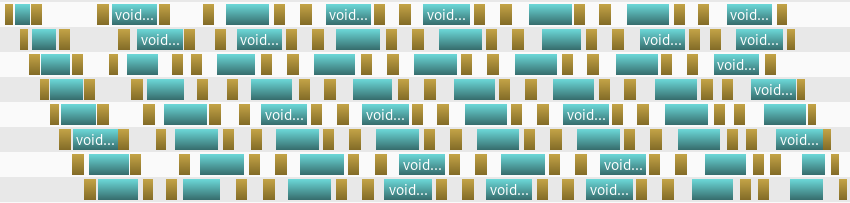
\includegraphics[width=.95\linewidth]{async648}
\end{figure}

\end{frame}




\begin{frame}[fragile]
\frametitle{Concurrency Example}
\begin{itemize}
	\item Implementation with streams and slices
\end{itemize}

\begin{lstlisting}
pinned_vector<T> h_data(N);
thrust::device_vector<T> d_data(N);

int sliceN = N / slices;
std::vector<cudaStream_t> streams(streamCount);

for (auto& s : streams)
{
    cudaStreamCreate(&s);
}
\end{lstlisting}
\end{frame}


\begin{frame}[fragile]
\frametitle{Concurrency Example}
\begin{itemize}
	\item Implementation with streams and slices
\end{itemize}

\begin{lstlisting}
for (int i = 0; i < slices; ++i)
{
    // Rotate through all streams
    auto& stream = streams[i % streamCount];
    T* d_slice   = d_data.data().get() + i * sliceN;
    T* h_slice   = h_data.data() + i * sliceN;

    cudaMemcpyAsync(d_slice, h_slice, sliceN * sizeof(T), 
    		cudaMemcpyHostToDevice, stream);
    process<T><<<iDivUp(sliceN, 128), 128, 0, stream>>>(
    		d_slice, sliceN);
    cudaMemcpyAsync(h_slice, d_slice, sliceN * sizeof(T), 
    		cudaMemcpyDeviceToHost, stream);
}
\end{lstlisting}
\end{frame}


\begin{frame}[fragile]
\frametitle{Concurrency Example Results}
\centering
\begin{tabular}{l|S|S}	
	\multicolumn{1}{c|}{\textbf{Method}} & \textbf{Time (ms)} & \textbf{Speed Up} \\
	\hline
	Initial 				& 13.55     & 1 \\
	Pinned Memory 1 Stream	& 9.50      & 1.426 \\
	Pinned Memory 2 Stream	& 6.87      & 1.97 \\
	Pinned Memory 4 Stream	& 5.57     & 2.43 \\
	Pinned Memory 8 Stream	& 4.94      & 2.74 \\
	Pinned Memory 16 Stream	& 4.60      & 2.94 \\
		Pinned Memory 8 Stream 64 Slices	& 4.41     & 3.07 \\
\end{tabular}
\\
\vspace{0.5cm}
\begin{itemize}
	\item[$\rightarrow$] With multiple streams and pinned memory the performance can be increased by a factor of 3 compared to the initial implementation
	\item[$\rightarrow$] \href{https://github.com/darglein/saiga/blob/master/samples/cuda/async/main.cu}{Full source code @ GitHub}
\end{itemize}

\end{frame}
\frame{
	\frametitle{Literature}
	%
	\begin{itemize}
		\item \href{https://docs.nvidia.com/cuda/}{Cuda Toolkit Documentation}
		\item \href{https://docs.nvidia.com/cuda/cuda-driver-api/}{CUDA driver API}
		\item \href{https://docs.nvidia.com/cuda/cuda-runtime-api/}{ CUDA runtime API}
	\end{itemize}
	
}





\end{document}



